\subsection{Các lớp chính}
\label{sec:core-objects}
Trước hết, chúng ta xây dựng các lớp chính. Các lớp được xây dựng với kiểu dữ liệu của ngôn ngữ \code{C++}, ta hoàn toàn có thể triển khai tương tự với các ngôn ngữ lập trình khác. Các kiểu số nguyên được sử dụng là \code{uint16\_t} với giá trị lớn nhất là $65535$ (đủ lớn để lưu số lượng khách hàng thực tế cũng như nhu cầu hay tải trọng của khách hàng...) để tiết kiệm bộ nhớ. Các kiểu số thực được sử dụng là \code{float} thay vì \code{double}. Đôi khi, trong một số bộ thư viện (như \code{Google OR-Tools} chẳng hạn), thay vì sử dụng số thực để lưu khoảng cách hay thời gian di chuyển giữa các yêu cầu hoặc giá trị hàm mục tiêu, số nguyên được sử dụng để tiết kiệm bộ nhớ cũng như tính toán nhanh hơn. Nếu cần nhiều hơn độ chính xác, ta có thể nhân tất cả với một hệ số ($1000$ chẳng hạn để đạt độ chính xác $3$ chữ số sau dấu chấm động) và chia lại khi nhận kết quả cuối cùng. Các lớp được liệt kê dưới đây cùng với giải thích cụ thể của từng thuộc tính và phương thức.

\begin{figure}[H] % places figure environment here   
	\centering % Centers Graphic
	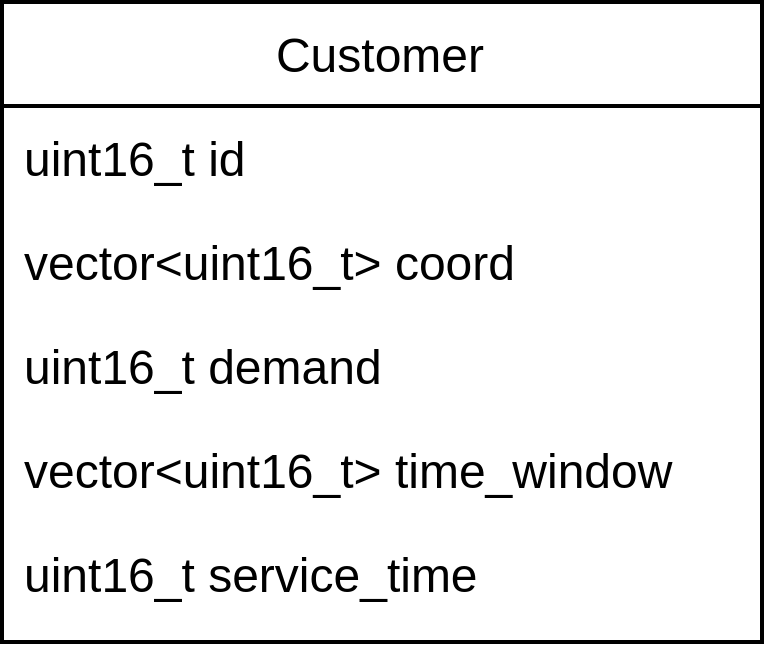
\includegraphics[width=0.35\textwidth]{figures/Customer.png}
	% \includesvg[scale=1]{figures/core-object}
	\caption{Lớp thuộc tính của khách hàng}
	\label{fig:fg_02}
\end{figure}

\code{Customer}: lớp lưu các thuộc tính của một yêu cầu. Đối với VRPTW, mỗi yêu cầu là một khách hàng (đơn).

\begin{itemize}
	\item[-] \code{id}: id của khách hàng.
	\item[-] \code{coord}: mảng lưu toạ độ của khách hàng (vĩ độ, kinh độ). Đôi khi chúng ta không cần quan tâm tới tọa độ của khách hàng mà quan tâm tới khoảng cách hoặc thời gian di chuyển giữa các khách hàng, nên thuộc tính này có thể không cần thiết đối với một số cấu hình trong thực tế.
	\item[-] \code{demand}: nhu cầu (về tải) của khách hàng.
	\item[-] \code{time\_window}: mảng lưu khung thời gian để phục vụ khách hàng. Mảng gồm 2 phần tử lần lượt là thời điểm sớm nhất và muộn nhất để phục vụ khách hàng.
	\item[-] \code{service\_time}: thời gian phục vụ khách hàng.
\end{itemize}


\code{CustomerRoute}: lớp lưu trạng thái về tuyến đường.
\begin{itemize}
	\item[-] \code{route\_idx}: id của tuyến chứa khách hàng.
	\item[-] \code{position}: vị trí của khách hàng trong tuyến.
\end{itemize}

\code{CustomerTime}: lớp lưu trạng thái về thời gian của yêu cầu.
\begin{itemize}
	\item[-] \code{arrival}: thời gian xe đến vị trí của khách hàng.
	\item[-] \code{complete}: thời gian xe hoàn thành phục vụ khách hàng.
\end{itemize}

\begin{figure}[H] % places figure environment here   
	\centering % Centers Graphic
	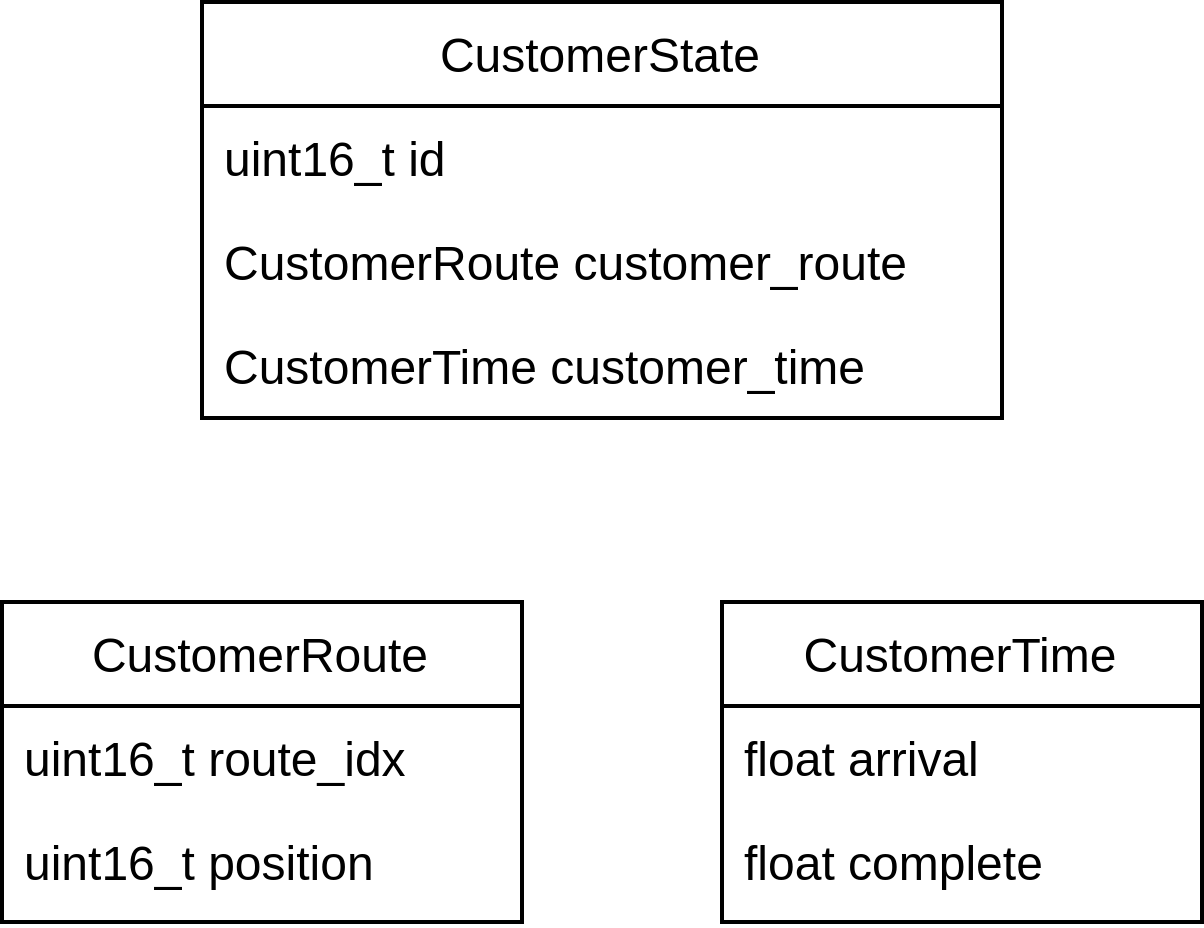
\includegraphics[width=0.6\textwidth]{figures/CustomerState.png}
	% \includesvg[scale=1]{figures/core-object}
	\caption{Lớp trạng thái của khách hàng}
	\label{fig:fg_03}
\end{figure}

\code{CustomerState}: lớp lưu trạng thái của khách hàng.
\begin{itemize}
	\item[-] \code{id}: id của khách hàng.
	\item[-] \code{customer\_route}: trạng thái về tuyến đường của khách hàng.
	\item[-] \code{customer\_time}: trạng thái về thời gian của khách hàng.
\end{itemize}

\begin{figure}[H] % places figure environment here   
	\centering % Centers Graphic
	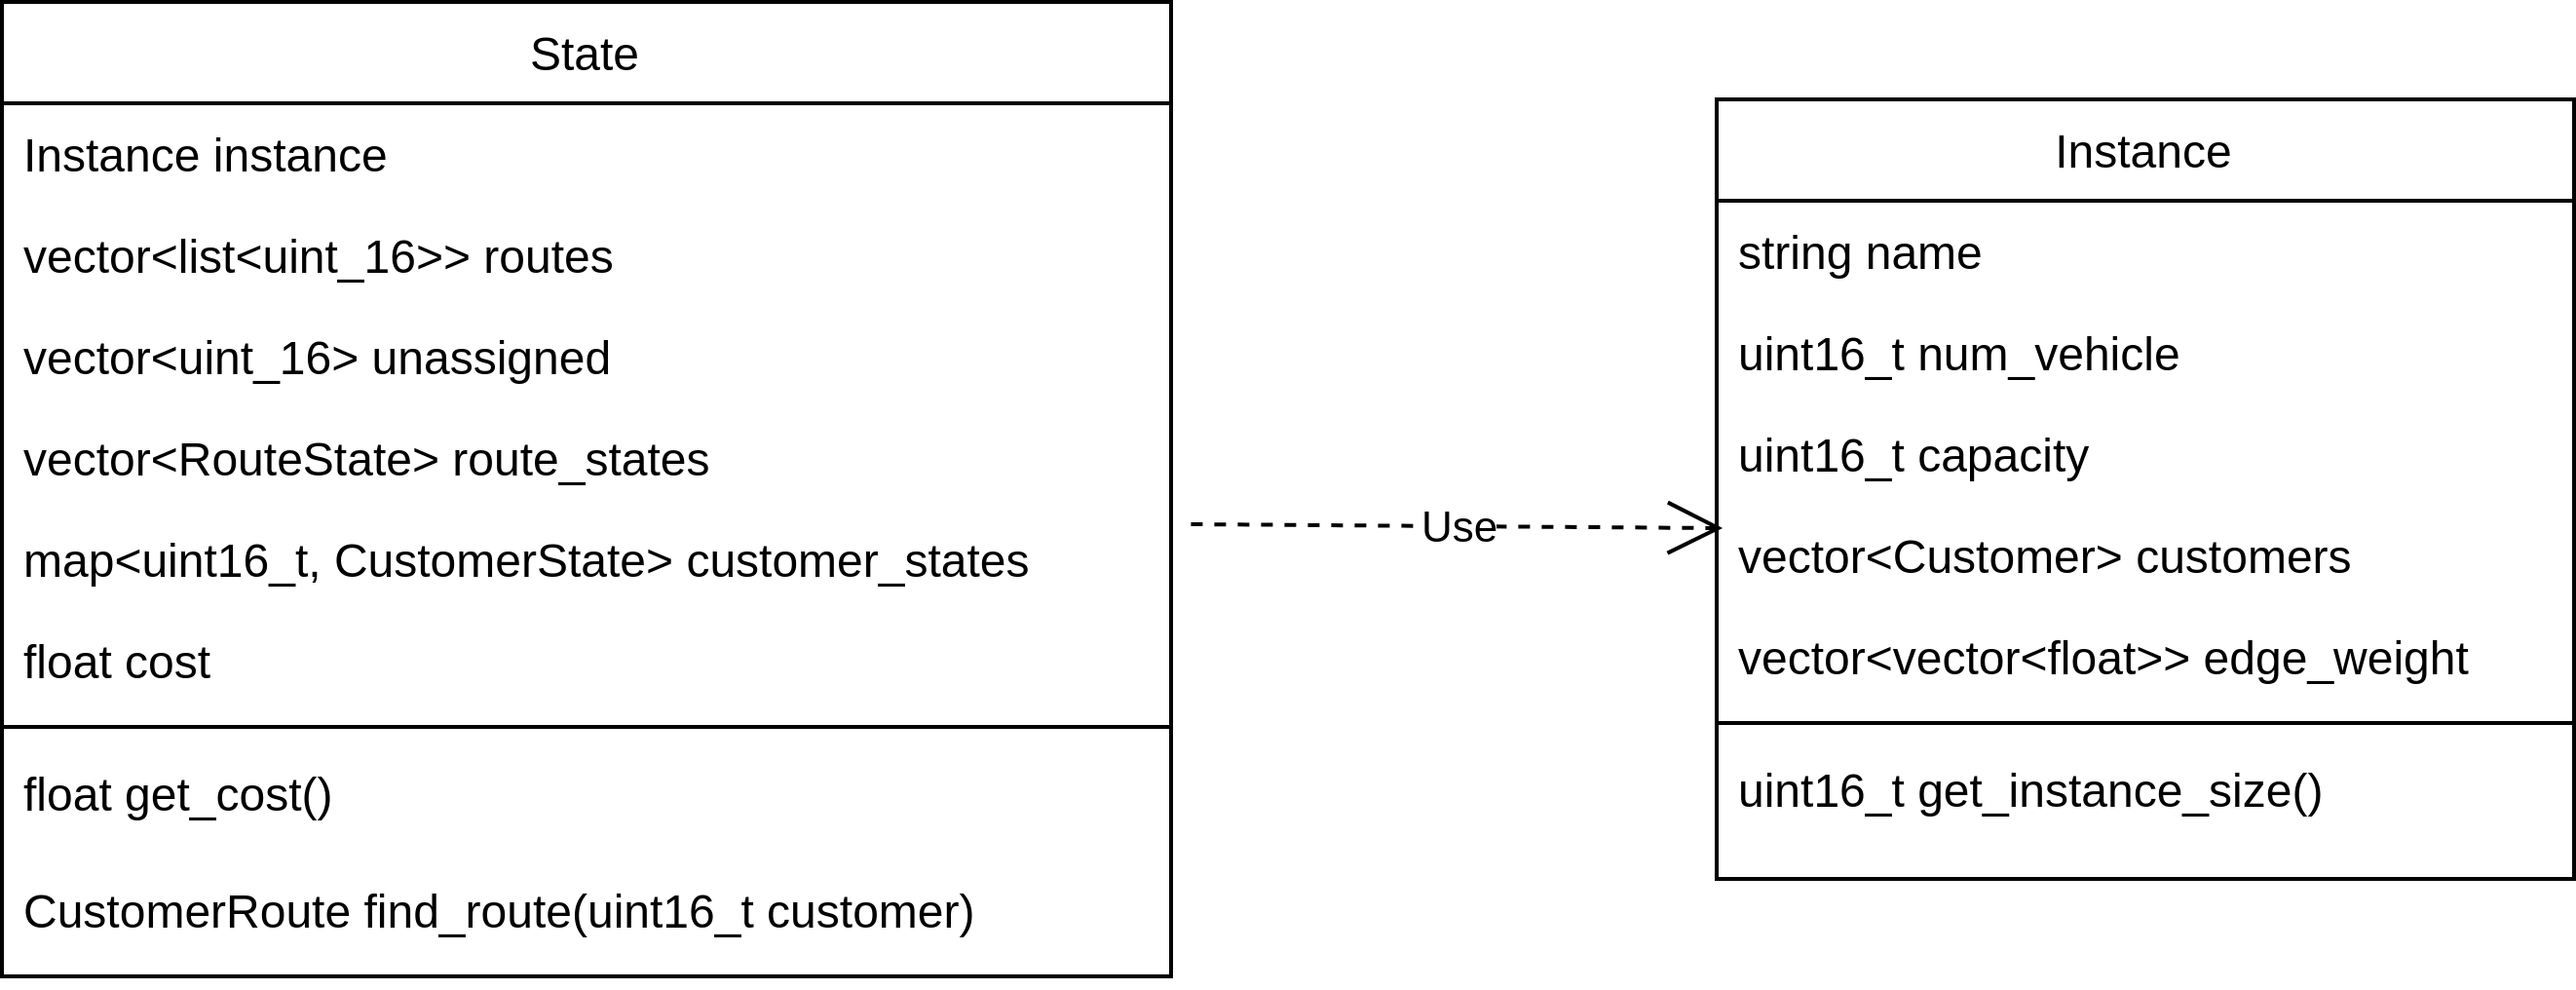
\includegraphics[width=1\textwidth]{figures/core-object.png}
	% \includesvg[scale=1]{figures/core-object}
	\caption{Lớp trạng thái của hệ}
	\label{fig:fg_04}
\end{figure}

\code{Instance}: lớp lưu cấu hình của bài toán.
\begin{itemize}
	\item[-] \code{name}: tên cấu hình (ví dụ \code{C101} trong tập Solomon (1987)).
	\item[-] \code{num\_vehicle}: số xe tối đa được sử dụng.
	\item[-] \code{capacity}: tải trọng của mỗi xe.
	\item[-] \code{customers}: mảng các yêu cầu.
	\item[-] \code{edge\_weight}: ma trận trọng số cạnh. Ma trận này có thể là ma trận khoảng cách hay thời gian di chuyển giữa các yêu cầu.
	\item[-] \code{get\_instance\_size()}: phương thức trả về kích thước của cấu hình (số khách hàng cộng với kho).
\end{itemize}

\code{State}: lớp lưu trạng thái của bài toán.
\begin{itemize}
	\item[-] \code{instance}: tham chiếu tới cấu hình bài toán.
	\item[-] \code{routes}: các tuyến đường. Các tuyến đường được tổ chức như một \code{vector} với mỗi thành phần là một \code{linked\_list}. Cấu trúc dữ liệu \code{linked\_list} được lựa chọn phù hợp với ALNS khi ta có thể  bỏ đi hoặc chèn thêm các yêu cầu vào giữa tuyến một cách nhanh chóng. Trong nhiều thuật toán khác, các yêu cầu được trao đổi giữa các tuyến thì \code{vector} là phù hợp hơn do ta có thể truy cập đến phần từ (yêu cầu) theo index rất nhanh mà không phải duyệt lần lượt từ đầu mảng giống như \code{linked\_list}. Việc sử dụng \code{linked\_list} cho ALNS là cực kì phù hợp, thao bỏ đi hay chèn thêm phần tử vào giữa tuyến nhanh hơn khoảng $250$ lần khi so sánh với việc sử dụng cấu trúc dữ liệu \code{vector}!
	\item[-] \code{unassigned}: danh sách các khách hàng chưa được phục vụ bởi bất kì xe nào.
	\item[-] \code{route\_states}: trạng thái của các tuyến, mỗi phẩn tử lưu lại tải và chi phí của tuyến.
	\item[-] \code{customer\_states}: trạng thái của các khách hàng.
	\item[-] \code{cost}: tổng chi phí của hệ (hay nghiệm) hiện tại.
	\item[-] \code{get\_cost()}: phương thức trả về cost hiên tại.
	\item[-] \code{find\_route(customer)}: phương thức trả về trạng thái của một khách hàng với đầu vào là id của khách hàng.
\end{itemize}